En el presente capitulo se presenta la institución y el problema que se aborda en el proyecto.

\section{Descripción de la institución}
\begin{itemize}
\item Nombre: Laboratorio de Sistemas Automatizados de Producción
\item Dirección: Avenida Collao 1202, Concepción, Chile
\item Encargado: Luis Vera
\item Rubro: Automatización
\item Teléfono: (41) 311 1137
\item Descripción: Laboratorio de ensayos para el desarrollo de disciplinas en el ámbito de la Automatización Industrial, Tecnologías Avanzadas de Manufactura, Gestión de la Producción, Robótica, Control Numérico y Visión por Computador.
\end{itemize}

\begin{figure}[ht]
\centering
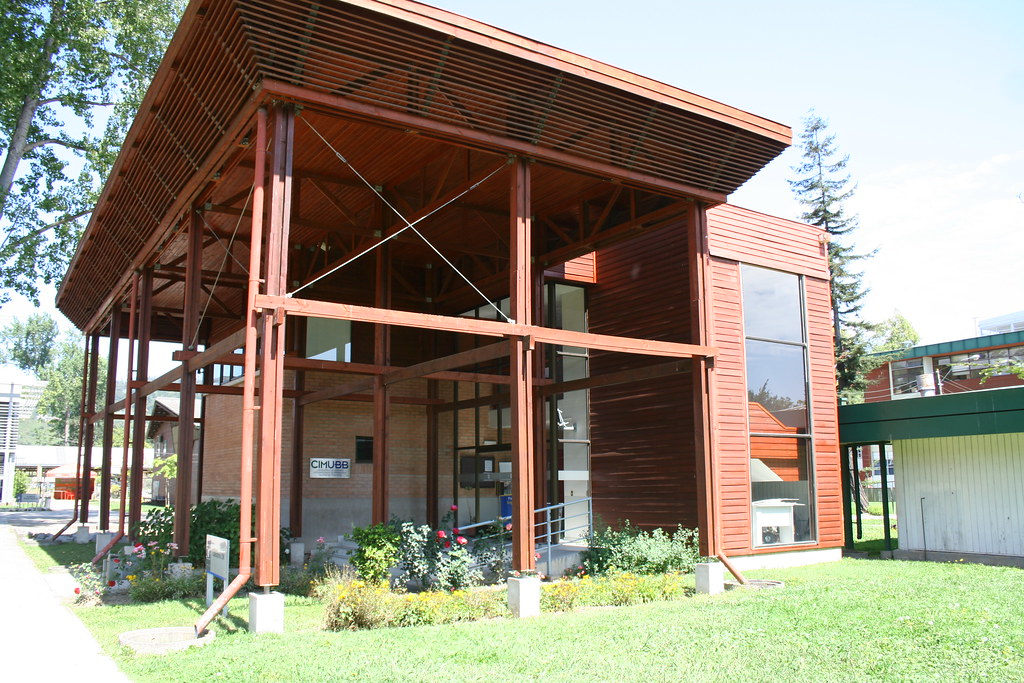
\includegraphics[width=13cm, height=6.8cm]{figures/cimubbfuera.jpg}
\caption{Edificio CIMUBB}
\label{fig:cimubbfuera}
\end{figure}

\clearpage
\section{Descripción del área de estudio}
La presente tesis tiene como objetivo principal abordar el área de estudio relacionada al laboratorio CIMUBB, el cual, por diversas razones, se puede no contar con acceso a este para realizar demostraciones prácticas. La limitación de acceso al laboratorio físico impide brindar una enseñanza completa y práctica a los estudiantes, ya que gran parte del aprendizaje depende de la interacción directa con la maquinaria y los experimentos que se encuentran en su interior.

Con el fin de superar esta limitación, se propone desarrollar un software de simulación que permita a los estudiantes experimentar y aprender de manera virtual dentro del entorno del laboratorio. El software de simulación debe recrear fielmente los equipos, las configuraciones y las condiciones experimentales presentes en el laboratorio real, brindando una experiencia inmersiva y cercana a la realidad.

La simulación se desarrolló utilizando tecnologías de vanguardia y siguiendo los estándares y protocolos establecidos en el campo de estudio correspondiente. Se diseñó una interfaz intuitiva y amigable para facilitar la interacción de los usuarios con los diferentes elementos del laboratorio virtual, permitiéndoles realizar experimentos, ajustar parámetros, recopilar datos y observar los resultados de sus acciones.

La creación de este software de simulación tiene como objetivo principal proporcionar una alternativa efectiva y accesible para la enseñanza y el aprendizaje en ausencia del acceso físico al laboratorio. De esta manera, se busca brindar a los estudiantes una plataforma que les permita adquirir conocimientos prácticos, desarrollar habilidades experimentales y comprender los conceptos teóricos en un entorno virtual seguro y controlado.

Se espera que esta iniciativa proporcione una solución innovadora que amplíe las posibilidades de enseñanza en el área de estudio, permitiendo a los educadores complementar las clases teóricas con experiencias prácticas simuladas. Además, se busca fomentar la autonomía y la experimentación activa por parte de los estudiantes, promoviendo el descubrimiento y la resolución de problemas dentro del contexto del laboratorio virtual.

En resumen, esta investigación se enfoca en el desarrollo de un software de simulación de laboratorio para superar la limitación de acceso físico, permitiendo así una enseñanza práctica y completa en el área de estudio correspondiente. Se espera que esta solución contribuya significativamente a la formación académica y profesional de los estudiantes, brindándoles una herramienta virtual valiosa y efectiva para su aprendizaje y desarrollo.

\clearpage

\section{Descripción de la problemática}
A los comienzos de la pandemia, el profesor encargado del laboratorio CIMUBB, Luis Vera, comienza a notar una necesidad para sus alumnos, una necesidad que siempre estuvo presente pero, para en esa fecha, nunca había sido tan clara ni tan vital como llegó a ser.

\begin{figure}[ht]
\centering
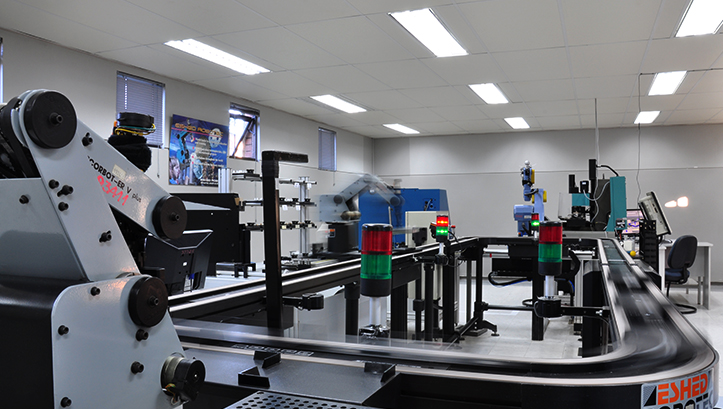
\includegraphics[width=13cm, height=6.1cm]{figures/cimubb.jpg}
\caption{Laboratorio CIMUBB}
\label{fig:cimubb}
\end{figure}

En la Figura ~\ref{fig:cimubb} se muestra una imagen del laboratorio CIMUBB, en el cual se llevan a cabo la entrega del conocimiento sobre la automatización, para la problemática del proyecto se enfoca en los brazos robóticos SCORBOT, los cuales son tres, siendo dos modelos diferentes.

\begin{figure}[ht]
\centering
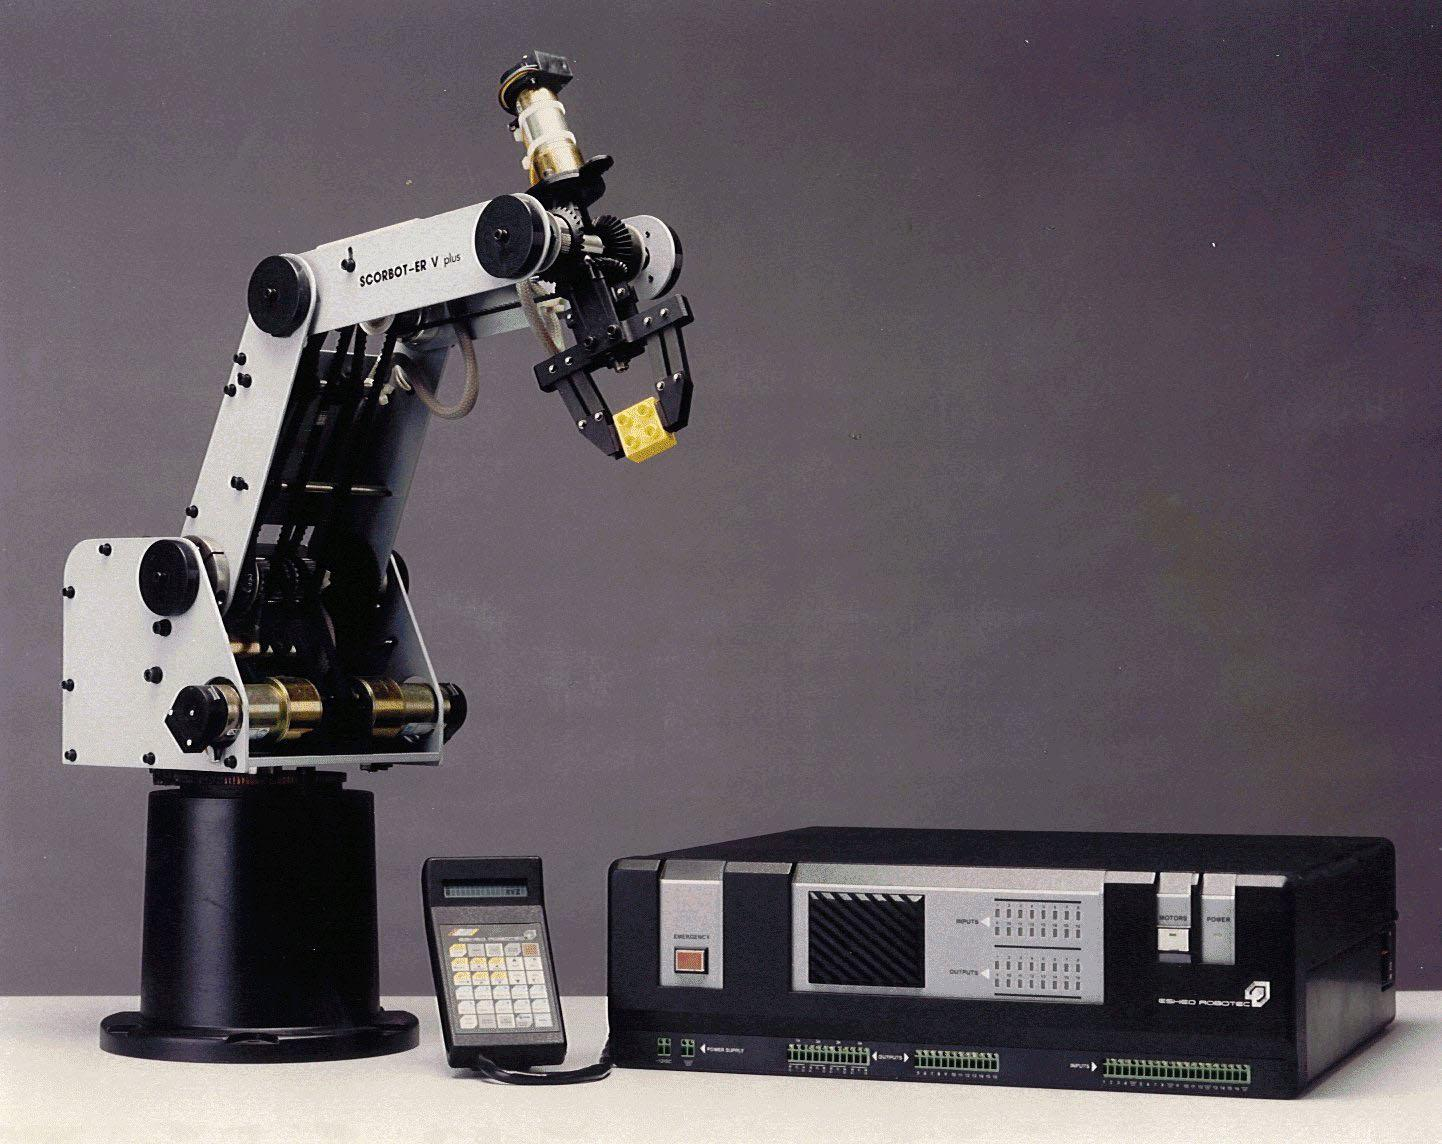
\includegraphics[width=13cm, height=6.1cm]{figures/scor5p.jpg}
\caption{SCORBOT ER V Plus}
\label{fig:scor5p}
\end{figure}

 En la Figura ~\ref{fig:scor5p} se presenta el brazo robótico SCORBOT ER V Plus, es un brazo de antigua generación, teniendo cinco ejes de movimiento para el brazo robótico estático y seis ejes para el que posee una cinta de movimiento lineal.

\clearpage

\begin{figure}[ht]
\centering
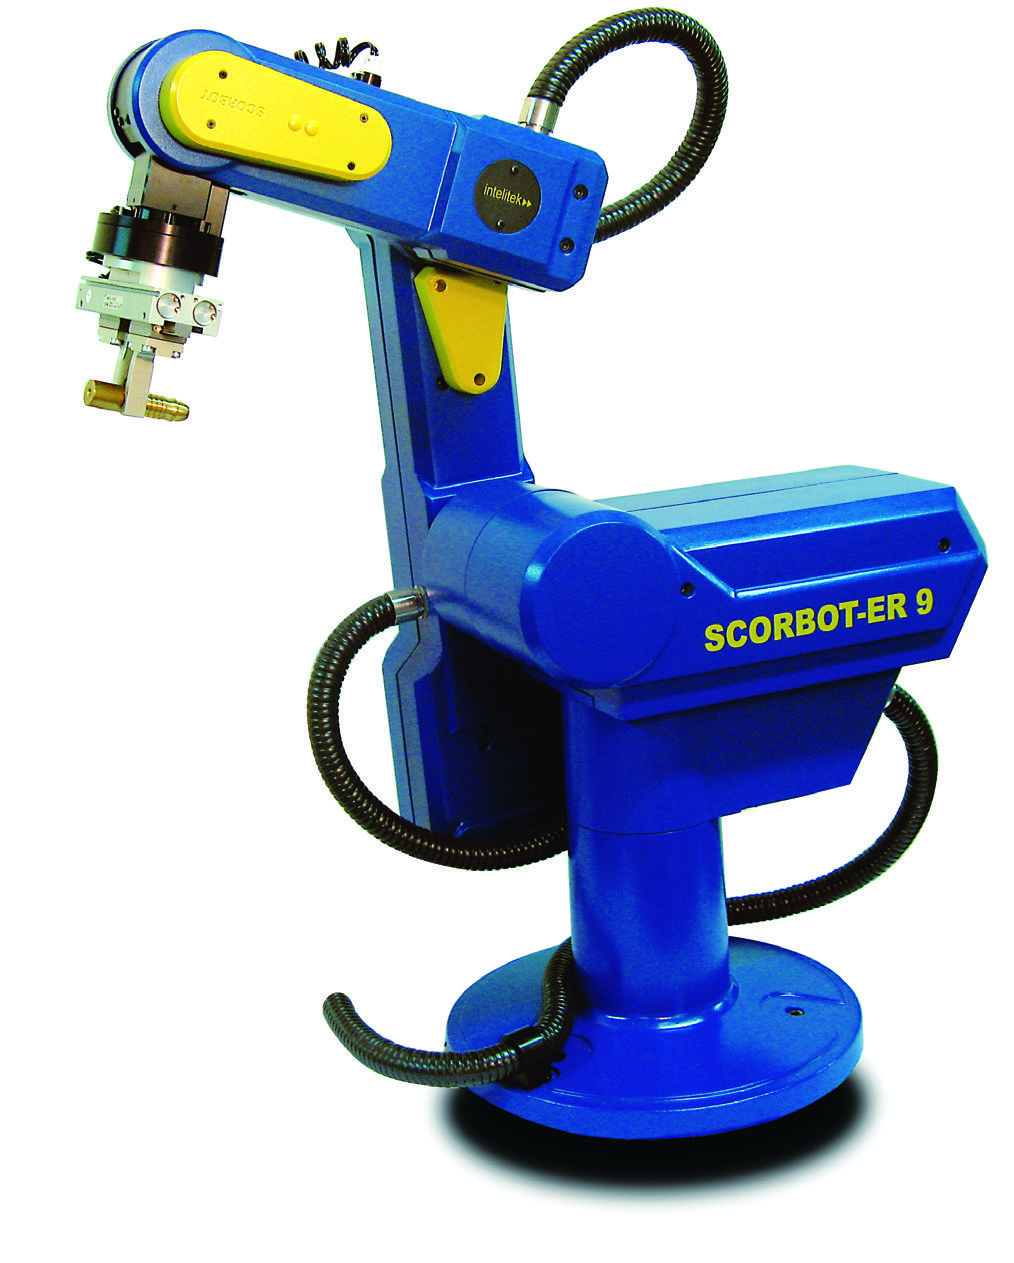
\includegraphics[width=13cm, height=12.5cm]{figures/scor9.jpg}
\caption{SCORBOT ER IX}
\label{fig:scor9}
\end{figure}

En la Figura ~\ref{fig:scor9} se presenta el brazo robótico SCORBOT ER IX, es una versión mejorada, la cual posee siete ejes de movimiento.

El laboratorio CIMUBB no cuenta con un entorno virtual, lo que dificulta significativamente el aprendizaje y la manipulación de los brazos robóticos SCORBOT cuando los estudiantes no pueden acceder físicamente al edificio. La falta de un entorno virtual restringe el acceso de los alumnos a prácticas y experimentos con los brazos robóticos, especialmente durante situaciones como cuarentenas, cortes de luz u otras fallas que requieren la presencia física de un supervisor o profesor.

La falta de acceso a un entorno virtual también limita la flexibilidad y disponibilidad para los estudiantes que deseen aprender sobre sistemas automatizados y brazos robóticos fuera de los horarios de clases regulares. Si el profesor no tiene acceso físico al laboratorio en un momento dado, los estudiantes se ven obligados a esperar hasta que el profesor pueda estar presente nuevamente en el lugar para realizar cualquier actividad relacionada con los brazos robóticos.